%%%%%%%%%%%%%%%%%%%%%%%%%%%%%%%%%%%%%%%%%%%%%%%%%%%%%%%%%%%%%%%%%%%%%%%%%%%%%%
%
% Section file included in main project file using \input{}
%
% Assumes that LaTeX2e macros and packages defined in cg_comp.sty are
%   available
%
%%%%%%%%%%%%%%%%%%%%%%%%%%%%%%%%%%%%%%%%%%%%%%%%%%%%%%%%%%%%%%%%%%%%%%%%%%%%%%

 \section{Tempering the Classical Guitar\label{app:temp}}

 \begin{figure}
  \centering
  \begin{subfigure}[b]{0.45\textwidth}
   \centering
   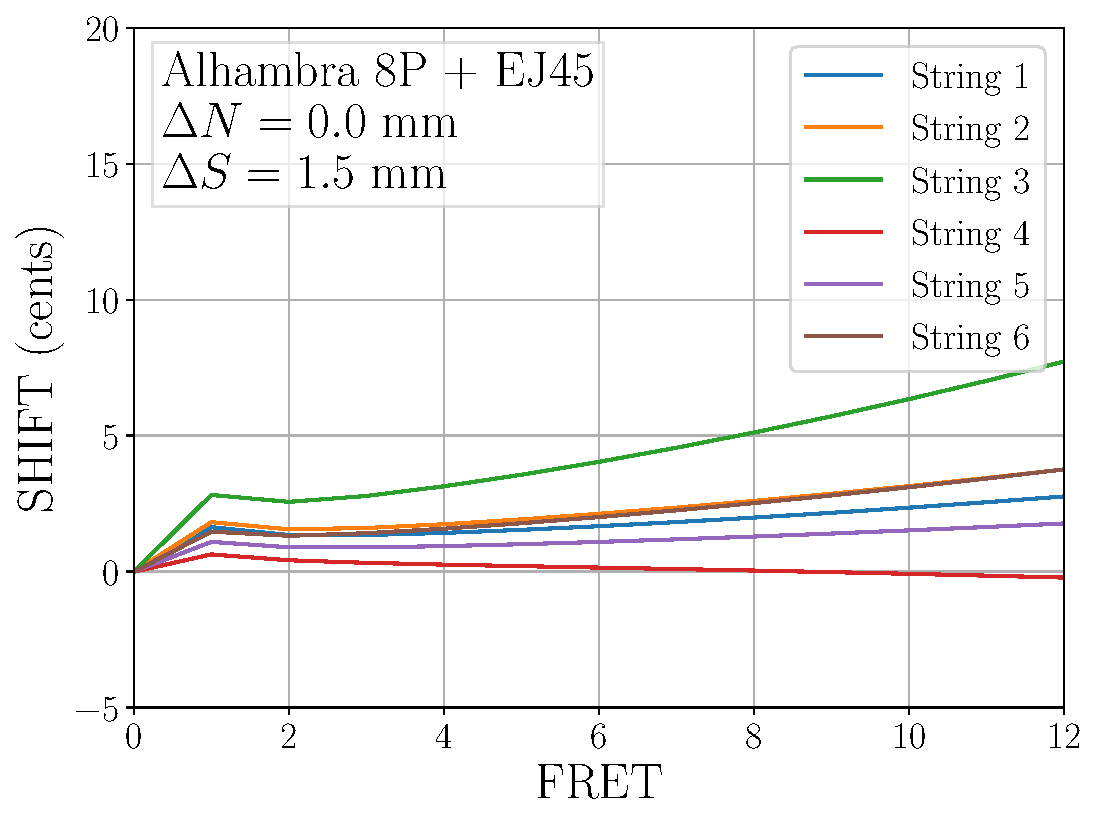
\includegraphics[width=3.25in]{figures/shift_alhambra8p_ej45_factory}
   \caption{Factory guitar --- 12-TET tuned}
   \label{fig:shift_alhambra8p_ej45_fact_temp}
  \end{subfigure}
  \hspace{0.25in}
  \begin{subfigure}[b]{0.45\textwidth}
   \centering
   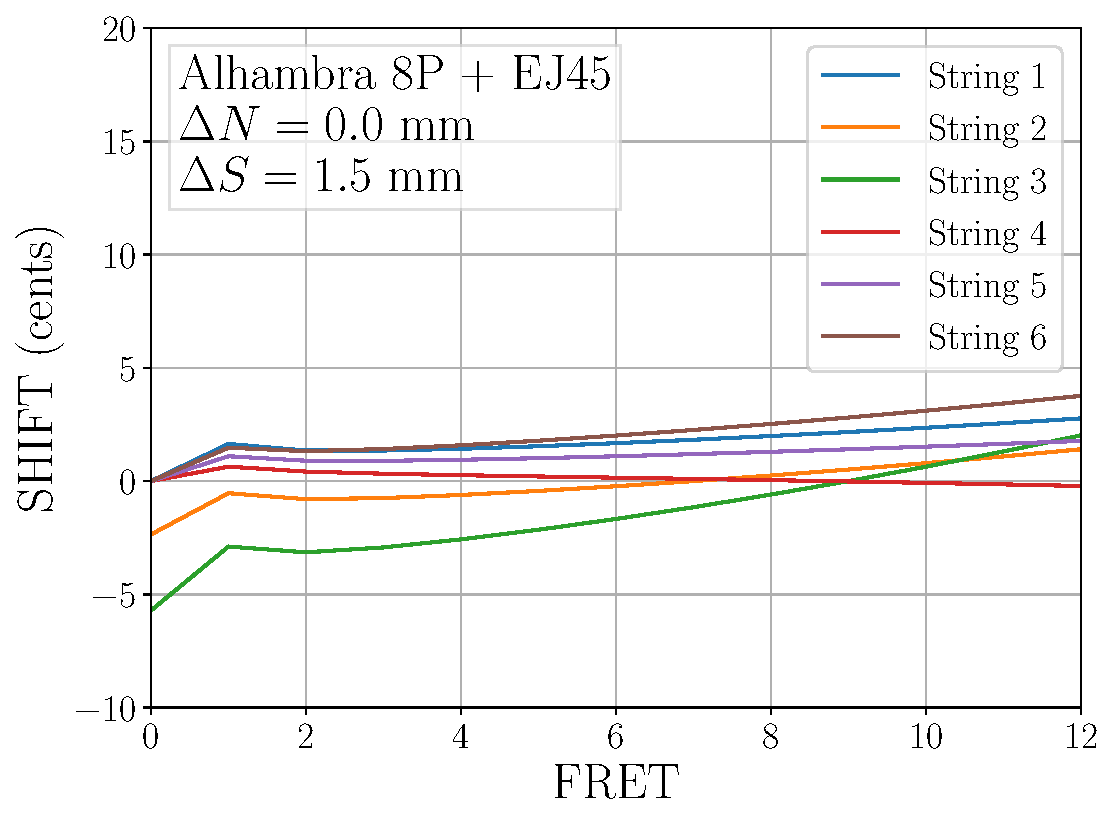
\includegraphics[width=3.25in]{figures/shift_alhambra8p_ej45_harmonic}
   \caption{Factory guitar --- harmonically tuned}
   \label{fig:shift_alhambra8p_ej45_harmonic}
  \end{subfigure}
  \caption{\label{fig:compensation_alhambra8p_ej45_temp} Frequency shift (in cents) for an Alhambra 8P guitar with D'Addario Pro-Arte Nylon Classical Guitar Strings -- Normal Tension (EJ45). Here we compare the factory guitar tuned to 12-TET with the same guitar harmonically tuned.}
 \end{figure}
